\documentclass{llncs}
\usepackage[latin1]{inputenc}
\usepackage[dvips]{epsfig}
\usepackage{alltt,amsmath,amssymb}
\usepackage{latexsym,pstricks,pst-node,pst-tree,boxedminipage,stmaryrd}
%\usepackage{times}
\usepackage{listings}
\def\lstlanguagefiles{lstlangjml.sty}
\lstloadlanguages{Jml}


 %% The frameit and Frameit environments formats text within a single
  %% Anything can be framed, including verbatim text.

\def\doframeit#1{\vbox{%
  \hrule height\fboxrule
    \hbox{%
      \vrule width\fboxrule \kern\fboxsep
      \vbox{\kern\fboxsep #1\kern\fboxsep }%
      \kern\fboxsep \vrule width\fboxrule }%
    \hrule height\fboxrule }}

\def\frameit{\smallskip \advance \linewidth by -7.5pt \setbox0=\vbox \bgroup
\strut \ignorespaces }

\def\endframeit{\ifhmode \par \nointerlineskip \fi \egroup
\doframeit{\box0}}

\newcommand{\alarm}[1]{\marginpar{#1}}

\begin{document}

\title{Precise analysis of memory consumption using program logics}
\author{Gilles Barthe\inst{1}\and Mariela Pavlova\inst{1}
\and Gerardo Schneider\inst{2}}
\institute{INRIA Sophia--Antipolis, France
\and Department of Informatics, University of Oslo, Norway}

\date{}

%%%%%%%%%%%%%%%%%%%%%%%%%%%%%%%%%%%%%%%%%%%%%%%%%%%%
%
% DEFINITIONS
%
%%%%%%%%%%%%%%%%%%%%%%%%%%%%%%%%%%%%%%%%%%%%%%%%%%

\newcommand{\bbb}{\mathbb{B}}
% moved here from carmel.tex
\newcommand{\spp}{\hspace{1.5cm}}


\newcommand{\semb}{\llbracket}
\newcommand{\seme}{\rrbracket}
\newcommand{\sem}[1]{ \semb #1 \seme}
\newcommand{\ia}[1]{ \semb #1 \seme}
\newcommand{\fia}[1]{ \mathcal{F}\semb #1 \seme}
\newcommand{\ria}[1]{ \mathcal{R}\semb #1 \seme}

\newcommand{\Coq}{{\sf Coq}}
\newcommand{\ocaml}{\textsc{ocaml}}

\newcommand{\memvar}{\text{Mem}}

\newcommand{\AbVal}{\widehat{\text{Val}}}
\newcommand{\Val}{{\text{Val}}}
\newcommand{\Stack}{{\text{Stack}}}
\newcommand{\AbStack}{{\widehat{\text{Stack}}}}
\newcommand{\SafeCallStack}{{\text{SafeCallStack}}}
\newcommand{\OneCall}{{\text{OneCall}}}
\newcommand{\Var}{{\text{Var}}}
\newcommand{\LocalVar}{{\text{LocalVar}}}
\newcommand{\AbLocalVar}{{\widehat{\text{LocalVar}}}}
\newcommand{\State}{{\text{State}}}
\newcommand{\Trace}{{\text{Trace}}}
\newcommand{\AbState}{{\widehat{\text{State}}}}
\newcommand{\progCount}{{\text{progCount}}}
\newcommand{\fieldName}{{\text{fieldName}}}
\newcommand{\methodName}{{\mathrm{methodName}}}
\newcommand{\MM}{{\methodName}}
\newcommand{\PP}{{\progCount}}
\newcommand{\className}{{\text{className}}}
\newcommand{\varName}{{\text{varName}}}
\newcommand{\Adress}{{\text{Adress}}}
\newcommand{\Instruction}{{\text{Instruction}}}
\newcommand{\InstAt}{{\text{InstAt}}}
\newcommand{\Constraint}{{\text{Constraint}}}
\newcommand{\St}{\widehat{\text{St}}}

\newcommand{\config}[1]{{\langle\!\langle #1 \rangle\!\rangle}}
\newcommand{\fram}[1]{{\left\langle #1 \right\rangle}}
\newcommand{\num}{{\text{num}}}
\newcommand{\reff}{{\text{ref}}}
\newcommand{\nul}{{\text{null}}}
\newcommand{\some}{{\text{some}}}
\newcommand{\nameClass}{{\text{nameClass}}}
\newcommand{\class}{{\text{class}}}
\newcommand{\newObject}{{\text{newObject}}}
\newcommand{\newArray}{{\text{newArray}}}
\newcommand{\lengthArray}{{\text{lengthArray}}}
\newcommand{\fieldValue}{{\text{fieldValue}}}
\newcommand{\Value}{{\text{Value}}}
\newcommand{\classes}{{\text{classes}}}
\newcommand{\RefValue}{{\text{RefValue}}}
\newcommand{\Location}{{\text{Location}}}
\newcommand{\methodLookup}{{\text{methodLookup}}}
\newcommand{\nbArgument}{{\text{nbArgument}}}
\newcommand{\nameMethod}{{\text{nameMethod}}}

\newcommand{\ClassName}{{{\text{ClassName}}}}
\newcommand{\FieldName}{{{\text{FieldName}}}}
\newcommand{\default}{{{\text{default}}}}
\newcommand{\END}{{{\text{END}}}}
\newcommand{\AbHeap}{{\widehat{\text{Heap}}}}

\newcommand{\Sinit}{{\mathcal{S}_{\mathit{init}}}}

\newcommand{\instructionAt}{{\text{instructionAt}}}


%\newcommand{\abs}{\mbox{${\cal S}\!\mathit{t}$}}
\newcommand{\abs}{\mbox{$\Sigma$}}
\newcommand{\addr}{\mbox{\em addr}}
\newcommand{\pc}{\mathit{pc}}
\newcommand{\stf}{{\mathit{sf}}}
\newcommand{\cl}{{\mathit{cl}}}

\newcommand{\analyze}{\text{\tt analyse}}
\newcommand{\Analyze}{\ensuremath{\mathit{Unbounded}(P)}}
\newcommand{\Program}{\text{Program}}

\newenvironment{constraint}{%
\noindent
\hspace{.3mm}$
\begin{array}[t]{l}}{%
\end{array}$\\[0.2cm]
}

\newenvironment{contraint}{%
\noindent
\hspace{1cm}$
\begin{array}[t]{l}}{%
\end{array}$\\[0.5cm]
}




\newcommand{\AbPop}{\widehat{\text{pop}}}
\newcommand{\AbPush}{\widehat{\text{push}}}
\newcommand{\AbTop}{\widehat{\text{top}}}
\newcommand{\AbBinop}{\widehat{\text{binop}}}
\newcommand{\AbApply}{\widehat{\text{apply}}}
\newcommand{\AbSubst}{\widehat{\text{subst}}}
\newcommand{\Num}{{{\text{Num}}}}
\newcommand{\AbNum}{{\widehat{\text{Num}}}}
\newcommand{\AbRef}{{\widehat{\text{Ref}}}}
\newcommand{\AbObject}{{\widehat{\text{Object}}}}
%\newcommand{\AbHeap}{{\widehat{\text{Heap}}}}
\newcommand{\Flow}{\text{\tt Flow}}

\newenvironment{myalltt}{\vspace*{-3pt}\begin{alltt}}{\end{alltt}\vspace*{-3pt}}

%%
%% Added by Gerardo (28/09/2004)
%%

\newcommand{\Rule}[2]
{
\frac{#1}
{
\begin{array}{l}
#2
\end{array}
}
}

\newcommand\Loop{\ensuremath{\mathit{Loop}}}
\newcommand\Pred{\ensuremath{\mathit{Pred}}}
\newcommand\BC{\ensuremath{\mathit{BC}}}
\newcommand\MutRec{\ensuremath{\mathit{MutRecR}}}
\newcommand\Rec{\ensuremath{\mathit{Rec}}}
\newcommand\Anc{\ensuremath{\mathit{Anc}}}
\newcommand\LoopCall{\ensuremath{\mathit{LoopCall}}}
\newcommand\Call{\ensuremath{\mathit{Call}}}
\newcommand\Q{\ensuremath{\mathit{Q}}}
\newcommand\tr{\ensuremath{\mathit{tr}}}

\newcommand\End{\ensuremath{\mathtt{end}}}
\newcommand\nop{\ensuremath{\mathtt{nop}}}
\newcommand\push{\ensuremath{\mathtt{push}}}
\newcommand\pop{\ensuremath{\mathtt{pop}}}
\newcommand\dup{\ensuremath{\mathtt{dup}}}
\newcommand\swap{\ensuremath{\mathtt{swap}}}
\newcommand\numop{\ensuremath{\mathtt{numop}}}
\newcommand\load{\ensuremath{\mathtt{load}}}
\newcommand\store{\ensuremath{\mathtt{store}}}
\newcommand\inc{\ensuremath{\mathtt{inc}}}
\newcommand\add{\ensuremath{\mathtt{add}}}
\newcommand\sub{\ensuremath{\mathtt{sub}}}
\newcommand\goto{\ensuremath{\mathtt{goto}}}
\newcommand\If{\ensuremath{\mathtt{if}}}
\newcommand\looksw{\ensuremath{\mathtt{lookupswitch}}}
\newcommand\tabsw{\ensuremath{\mathtt{tableswitch}}}
\newcommand\newarray{\ensuremath{\mathtt{newarray}}}
%\newcommand\default{\ensuremath{\mathtt{default}}}
\newcommand\new{\ensuremath{\mathtt{new}}}
\newcommand\checkc{\ensuremath{\mathtt{checkcast}}}
\newcommand\getst{\ensuremath{\mathtt{getstatic}}}
\newcommand\putst{\ensuremath{\mathtt{putstatic}}}
\newcommand\instof{\ensuremath{\mathtt{instanceof}}}
\newcommand\getfd{\ensuremath{\mathtt{getfield}}}
\newcommand\getfdt{\ensuremath{\mathtt{getfield this}}}
\newcommand\putfd{\ensuremath{\mathtt{putfield}}}
\newcommand\invdef{\ensuremath{\mathtt{invokedefinite}}}
\newcommand\invvir{\ensuremath{\mathtt{invokevirtual}}}
\newcommand\invint{\ensuremath{\mathtt{invokeinterface}}}
\newcommand\return{\ensuremath{\mathtt{return}}}
\newcommand\arrlh{\ensuremath{\mathtt{arraylength}}}
\newcommand\arrld{\ensuremath{\mathtt{arrayload}}}
\newcommand\arrst{\ensuremath{\mathtt{arraystore}}}
\newcommand\throw{\ensuremath{\mathtt{throw}}}
\newcommand\jsr{\ensuremath{\mathtt{jsr}}}
\newcommand\ret{\ensuremath{\mathtt{ret}}}
\newcommand\this{\ensuremath{\mathtt{this}}}
\newcommand\instr{\ensuremath{\mathtt{instr}}}
\newcommand\const{\ensuremath{\mathtt{const}}}
\newcommand\Array{\ensuremath{\mathsf{array}}}
\newcommand\Int{\ensuremath{\mathsf{int}}}
\newcommand\byte{\ensuremath{\mathsf{byte}}}
\newcommand\short{\ensuremath{\mathsf{short}}}
\newcommand\bool{\ensuremath{\mathsf{bool}}}
\newcommand\Ctxt{\ensuremath{\mathsf{Ctxt}}}

\newcommand\warn{\ensuremath{<!>}}
\newcommand\trace{\overline{s}}
\newcommand\defi{\stackrel{\mathrm{def}}{=}}
\newcommand\lub{\sqcup}

\newcommand\Size{\ensuremath{\mathit{Size}}}
\newcommand\Pre{\ensuremath{\mathrm{Pre}}}
\newcommand\Post{\ensuremath{\mathrm{Post}}}
%\newcommand\old{\ensuremath{\backslash\mathrm{old}}}

%%%%%%%%%%%%%%%%%%%%%%%%%%%%%%%%%%%%%%%%%%%%%%%%%%%%%%%
%%
%% Mariela's definitions
%%
%%%%%%%%%%%%%%%%%%%%%%%%%%%%%%%%%%%%%%%%%%%%%%%%%%%%%%%

\newcommand{\blockm}[1]{ $b^{#1}$ }
\newcommand{\pathm}[2]{\blockm{#1} $\ll^{*}$ \blockm{#2} }

\newtheorem{defn}{Definition}

%%%%%%%%%Specification commands
\newcommand{\annotation}{BML}
\newcommand{\Apredicate}{\textit{P}}
\newcommand{\predicate}{\mathcal{P}}
\newcommand{\expression}{\mathcal{E}}
\newcommand{\requires}{\texttt{requires}}
\newcommand{\ensures}{\texttt{ensures}}
\newcommand{\exsures}[1]{\texttt{exsures(#1)}}
\newcommand{\assert}{\texttt{assert}}
\newcommand{\invariant}{\texttt{invariant}}
\newcommand{\variant}{\texttt{variant}}

\newcommand{\declare}{\texttt{declare}}
\newcommand{\ghost}{\texttt{Model}}
\newcommand{\ghostSet}{\texttt{set}}
\newcommand{\modifies}{\texttt{modifies}}
\newcommand{\ensemble}[2]{#1 .. #2}
\newcommand{\maxIter}[1]{ iter^#1 }
\newcommand{\progLoop}[1]{\textit{#1}}
\newcommand{\memConsAt}[1]{\Mem^l}
\newcommand{\method}{\textit{m}}
\newcommand{\atState}[2]{#1^{#2} }

\newcommand{\Mem}{\texttt{MemUsed}}
\newcommand{\old}{\texttt{old}}
\newcommand\Max{\ensuremath{\texttt{Max}}}
\newcommand{\allocated}[1]{allocPath(#1)}
\newcommand{\srcCode}[1]{\texttt{#1}}
\newcommand{\local}[1]{\texttt{localVar}(#1)}



%%%%%%%%%%%% allocation function
\newcommand{\visited}{\texttt{visited}}
\newcommand{\true}{\textit{true}}
\newcommand{\false}{\textit{false}}

\newcommand{\instrAt}[1]{i_{#1}}
%\newcommand{\instanceOfAlloc}[1]{instanceOfAllocates( #1 )}

\newcommand{\allocInstance}[1]{\texttt{allocInstance(#1)}}
\newcommand{\allocLoop}[1]{loopConsumption(#1)} % function that returns directly the allocations done by a loop : multiplied by the max iterations it can do
\newcommand{\allocMethod}[1]{\texttt{methodConsumption(#1)}} % returns the allocations done in a method
\newcommand{\allocLoopWithEnd}[2]{alloc\_loop\_path(#1 , #2)} % returns the allocations done in a loop for a particular path that starts at the start instruction of a loop and that % ends with an insstruction that leads back to the start instructions

\newcommand{\allocIns}[1]{alloc\_instr(#1)} % function that returns that the allocation by the argument

\newcommand{\numLoop}[1]{\textit{numberLoop}(#1)}
\newcommand{\loopEndsSet}[1]{loopEndSet(#1)}
\newcommand{\loopSet}[1]{loopSet(#1)}
\newcommand{\loopEntry}[1]{entry(#1)} % predicate that says that the instruction is an entry to a loop

\newcommand{\backedge}[2]{backedge(#1,#2)} % the start of the backedge  and the end of the backedge


\newcommand{\wpi}[3]{ \rm{wp}( \srcCode{#1}, #2, #3) } % wp for instructions
\newcommand{\wpExe}[1]{ \rm{wp}(#1) } % wp for blocks
\newcommand{\normalPost}{\psi^{n}}
\newcommand{\excPost}{\psi^{exc}}

\newcommand{\stack}[1]{St(#1)}
\newcommand{\topStack}{c}
\newcommand{\javaNull}{null}
\newcommand{\Ref}[1]{ref_{#1} }
\newcommand{\NULL}{\texttt{null}}
\newcommand{\substitution}[2]{[ #1 \leftarrow #2] }


\newcommand{\prevIns}[1]{prev(#1 )}
\newcommand{\nextIns}[1]{next(#1 )}
\newcommand{\targetIns}[1]{target(#1)}



%%%%%%%%%%%%%%%%%%%%%%%%%%%%%%%%%%%%%%%%%%%%%%%%%%%%%
\newcommand{\todo}[1]
{\marginpar{\baselineskip0ex\rule{2,5cm}{0.5pt}\\[0ex]{\tiny\textsf{#1}}}}


\maketitle

\abstract{Memory consumption policies provide a means to control
resource usage on constrained devices, and play an important role
in ensuring the overall quality of software systems, and in
particular resistance against resource exhaustion attacks. Such
memory consumption policies have been previously enforced through
static analyses, which yield automatic bounds at the
cost of precision, or run-time analyses, which incur an overhead
that is not acceptable for constrained devices.

In this paper, we study the use of logical methods to specify and
verify statically precise memory consumption policies for Java
bytecode programs. First, we demonstrate how the Bytecode Modeling
Language BML (a variant of the Java Modeling Language JML tailored to
bytecode) can be used to specify precise memory consumption policies
for (sequential) Java applets, and how verification tools can
be used to enforce such memory consumption policies. Second, we
consider the issue of inferring some of the annotations required to
express the memory consumption policy. We report on an inference
algorithm and illustrate its applicability on non-trivial examples.


Our broad conclusion is that logical methods provide a suitable means
to specify and verify expressive memory consumption policies, with a
minimal overhead.}




%\vspace*{0.1cm}
%\noindent {\bf Keywords:}

\section{Introduction}

%\input BML/cmdBML.tex

\newcommand{\code}{\textit{code}}
\newcommand{\indexComp}{\textit{index}}





\section{Introduction} \label{bcsl}
This section presents a bytecode level specification language, called for short BML and a compiler from a
 subset of the high level Java specification language JML to BML. 

% motivation

 Before going further, we discuss what advocates the need of a low level specification language.
Traditionally, specification languages were tailored for high level languages.  
Source  specification allows to express complex functional or security properties about programs.
Thus, they are / can successfully be used 
for software audit and validation. Still, source specification in the context of mobile code does not help a lot for several reasons.


First, the executable / interpreted code  may not be accompanied by its specified  source. Second, it is more reasonable for the 
code receiver to check the executable code than its source code, especially if he is not willing to trust the compiler. 
Third, if the client has complex requirements and even if the code respects them, in order to establish them, 
the code should be specified. Of course, for properties like well typedness this specification can be inferred automatically,
but in the general case this problem is not decidable. 
Thus, for more sophisticated policies, an automatic inference will not work.

 It is in this perspective, that we propose to make the Java
bytecode benefit from the source specification by defining the BML language and a compiler from JML towards BML.    

% what does the language support?
 BML supports the most important features of JML. Thus, we can express functional properties of Java
 bytecode programs in the form of method pre and postconditions, class and object invariants, assertions
 for particular program points like loop invariants. To our knowledge BML does not have predecessors that are tailored 
 to Java bytecode.  

 In section \ref{BCSLprelim}, we give an overview of the main features of JML. A detailed overview of BML is given in section \ref{BCSLgrammar}.  
  As we stated before, we support also a compiler from the high level specification language JML into BML. The 
 compilation process from JML to BML is discussed in section  \ref{BCSLcompile}.
 The full specification of the new user defined Java attributes in which the JML specification is compiled is given in the appendix.






\section{Preliminaries}\label{sec:prelim}
\newtheorem{defEdge}{Definition}[section]
\newtheorem{defLoop}[defEdge]{Definition}
\newtheorem{defInter}[defEdge]{Definition}
\newtheorem{defExc}[defEdge]{Definition}
\newtheorem{defInv}[defEdge]{Definition}
\newtheorem{defModif}[defEdge]{Definition}

\newtheorem{propPath}{Lemma}[section]

\section{Representing bytecode programs as control flow graphs}\label{prelim}

This section will introduce a formalization of an unstructured program in terms of a control flow graph.
The notion of a loop in a bytecode program will be also defined.
Performing analysis on programs written in  structured languages, is usually easier than performing the same analysis 
on unstructured programs. In particular, source loops in a method body correspond to a syntactic construction which is not the 
case for loops in methods on bytecode level. In order to discover a loop in a bytecode program we first need to define 
what is a bytecode program. Note that in the following, by a  bytecode program we mean a method body.

Every method \methodd \ has an array of bytecode instructions \methodd.\body \  which we already introduced in Section \ref{clazz}.
The $k-th$ instruction in the bytecode array $\methodd.\body$ is  denoted with $\methodd.\body[k]$.
 We assume that the method body has exactly one entry point
 (an entry point instruction is the instruction at which an execution of a method starts) which is the first
 element in the method body
$\methodd.\body[0]$.
The array of bytecode instructions of a method \methodd \ determine an oriented graph $G( V , \execRel ) $ in which the vertices are the instructions of the method body,
i.e. $$ V = \{ ins \mid \exists k,  0 \leq k < \methodd.\body.length \wedge ins = \methodd.\body[k] \}$$
The following definition defines the set of edges in the control flow graph.
\begin{defEdge}[Edge in control flow graph]\label{defEdge} 
 The set of edges $\execRel$ is a relation between the vertices elements
$$ \execRel : V * V $$ and is defined  as follows:
$$ \begin{array}{l} (\methodd.\body[j], \methodd.\body[k]) \in \execRel \\
   \iff \\
   \begin{array}{l} \methodd.\body[j] \neq \return \wedge( \\
                    \methodd.\body[j] = \ifCond \ k \vee \\
		    \methodd.\body[j] = \goto \ k \ \vee \\
		    \methodd.\body[j] \neq \goto \wedge  k = j+1 \ \vee \\ 
		    \methodd.\body[j] = \putfield \wedge \findExcHandler{ \NullPointerExc}{j}{\methodd.\excHandlerTable} = k \ \vee \\
		    \methodd.\body[j] = \getfield \wedge \findExcHandler{ \NullPointerExc}{j}{\methodd.\excHandlerTable} = k \ \vee \\
		    \methodd.\body[j] = \arrstore \wedge \findExcHandler{ \NullPointerExc}{j}{\methodd.\excHandlerTable} = k \ \vee \\
                    \methodd.\body[j] = \arrstore \wedge \findExcHandler{\ArrIndexOutOfBoundExc  }{j}{\methodd.\excHandlerTable} = k \ \vee \\
		    
		    \methodd.\body[j] = \arrload \wedge \findExcHandler{ \NullPointerExc}{j}{\methodd.\excHandlerTable} = k \ \vee \\
                    \methodd.\body[j] = \arrload \wedge \findExcHandler{\ArrIndexOutOfBoundExc  }{j}{\methodd.\excHandlerTable} = k \ \vee \\
		    \methodd.\body[j] = \invoke \ \mbox{\rm \texttt{n}} \wedge \findExcHandler{\NullPointerExc }{j}{\methodd.\excHandlerTable} = k \ \vee \\
		     \methodd.\body[j] = \invoke \ \mbox{\rm \texttt{n}} \wedge \forall \mbox{\rm\texttt{Exc}}, \exists s , \mbox{\rm \texttt{n}}.\exceptions[s ] = \mbox{\rm\texttt{Exc}} \wedge  \\
	\phantom{\methodd.\body[j] = \invoke } \findExcHandler{\mbox{\rm\texttt{Exc}} }{j}{\methodd.\excHandlerTable} = k \ \vee \\	    
		    \methodd.\body[j] = \athrow  \wedge \forall \mbox{\rm\texttt{Exc}}, \findExcHandler{\mbox{\rm\texttt{Exc}} }{j}{\methodd.\excHandlerTable} = k \ \vee \\
		    %\methodd.\body[j] = \athrow  \wedge \findExcHandler{\NullPointerExc }{j}{\methodd.\excHandlerTable} = k \vee 
		    
		    )
   \end{array} 
\end{array}$$
\end{defEdge}
From the Def. \ref{defEdge} follows that there is an edge between two vertices $\methodd.\body[j]$ and  $\methodd.\body[k]$ if they may execute immediately one after another.
 We say that $\methodd.\body[j]$ is a predecessor of $\methodd.\body[k]$ and that  $\methodd.\body[k]$ is a successor of  $\methodd.\body[j]$.
 The definition states the \return \  instruction  does not have successors.
If  $\methodd.\body[j ]$ is the jump instruction $ \ifCond \ k $ then  its successors are the instruction at index $k$ in the method body   
$\methodd.\body[k]$ and the instruction and the instruction $\methodd.\body[j + 1 ]$. 
From the definition, we also get that every instruction which potentially may throw an exception of type \texttt{Exc}
has as successor the first instruction of the exception handler that may handle the exception type \texttt{Exc}. For instance, a successor
of the instruction $\putfield$ is the exception handler entry point which can handle  the \NullPointerExc \ exception. 
The possible successors of the instruction $\athrow$ are the entry point of any  exception handler  in the method \methodd.
In the following, we will rather use the infix notation $\methodd.\body[j] \execRel \methodd.\body[k]$.
% We will also use the notation $\next{\methodd.\body[j] }$ for denoting the successor of   $\methodd.\body[j]$ in a given execution path.


We assume that the control flow graph of every method is reducible, i.e. every loop has exactly one entry point. This actually is admissible
as it is rarely the case that a compiler produce a bytecode with a non reducible control flow graph and the practice shows that even hand written
code is usually reducible. However, there exist algorithms to transform a non reducible control flow graph into a reducible one. 
For more information on program control flow graphs, the curious reader may refer to \cite{ARUCom1986}.
The next definition identifies backedges in the reducible control flow graph ( intuitively, the edge that goes 
from an instruction in a given loop in the control flow graph to the loop entry)  with the special execution relation $\execRel^l$ as follows:
 
\begin{defLoop}[Backedge Definition]
\label{defLoop}
Assume we have the method \methodd \ with body \methodd.\body \ which determine the control flow graph $G(V, \execRel) $.  We assume also 
that the entry point of $G$ is the vertice  $\methodd.\body[0]$.
 In such a graph $G$, we say that $\ins{loopEntry}$ is a loop entry instruction and $\ins{f}$ is a loop end instruction
 of the same loop if the following conditions hold:
\begin{itemize}
\item for every execution path $P$ from $\methodd.\body[0]$ to  $\ins{f}$:   $P~=~\methodd.\body[0] \execRel^{+} \ins{f}$
 there exists a subpath which is a prefix of $P$  $subP = \methodd.\body[0] \execRel^{*} \ins{loopEntry}$ such that $\ins{f} \notin  \ subP  $
%every path in the control flow graph starting at the entry point $\methodd.\body[0]$  that reaches $\ins{f}$, passes before reaching $\ins{f}$
% through  $\ins{loopEntry}$ 
\item there is a path in which $\ins{loopEntry}$  is executed immediately after the execution of $\ins{f}$ ( $\ins{f} \execRel \ins{loopEntry}$)
\end{itemize}
We denote the execution relation between $\ins{f}$ and  $\ins{loopEntry}$ with \\
$\ins{f} \execRel^l \ins{loopEntry}$ and we say that $  \execRel^l $  is a backedge. 
\end{defLoop}
We illustrate the upper definition with the control flow graph of the example from Fig. \ref{replaceSrc} in Fig. \ref{ctrlflow}.
In the figure, we rather show the execution relation between basic blocks which is a standard notion denoting a sequence of instructions which execute sequentially
and  where only the last one may be a jump and the first may be a target of a jump. 
The black edges represent a sequential execution relation, while dashed edges represent a backedge, i.e. the edge which stands for the execution
relation between a final instruction (instruction at index \texttt{18}) in the bytecode cycle and the entry instruction of the cycle (instruction at index \texttt{19}).  

% Note that from now on, we are interested in  control flow graphs with the following properties:

% \begin{itemize}
%  \item the control flow graph is reducible
 % \item an exception handler cannot be n
% \end{itemize}
 
\begin{figure}[ht!]
\begin{center}
%\includegraphics{bc.eps}
\epsfig{file=figs/bc.eps, height=5in,  width=1.5in}
\caption{{ \sc The control flow graph of the source program from Fig.\ref{replaceSrc}} }
\label{ctrlflow}
\end{center}
\end{figure}

%The next lemma states a property about execution paths in a control flow graph that contains backedges. This lemma will be used in the proof of correctness
% of our calculus in section \ref{proof}.
% \begin{propPath} \label{propPath}
% Let's have a control flow graph with an entry point instruction $\methodd.\body[0]$ and two instructions $\ins{loopEntry}$ and  
% $\ins{f}$ such that  \\
% $\ins{f}~\execRel^l~\ins{loopEntry}$. If there exists an execution path $P$ from $\methodd.\body[0]$ to  $\ins{f}$:   $P~=~\methodd.\body[0] \execRel^{+} \ins{f}$
% then there exists a subpath which is a prefix of $P$  $subP = \methodd.\body[0] \execRel^{*} \ins{loopEntry}$ such that $\ins{f} \notin  \ subP  $ 
% \end{propPath} 


%Once we have defined what a loop means in a control flow graph, we want also to define what a loop invariant means. 

%\begin{defInv}[Loop Invariant]\label{defInv}
%An invariant is an assertion which accompanies a backedge  in a bytecode control flow graph. Every backedge is accompanied 
%by an invariant. We denote an invariant with $\invariant$. If a backedge  $\execRel^{l}$ is accompanied by an invariant $\invariant$ 
%then $\invariant$ holds in every state in which an execution path passes through  the edge $\execRel^{l}$.    
%\end{defInv}

%We also assume that loop entries are provided with the locations \modifLoop \ that a loop may modify. 
%The interest of having the set of the locations that may be modified by a loop will be seen later when defining the weakest precondition
%predicate transformer.


% \begin{defModif}[Loop Modifies]\label{defModif} Every loop entry instruction $\ins{loopEntry}$ with
%a set of locations $\modifLoop = \{ mod_i \mid  i = 1 .. s\}$ whose meaning is the following: any two states $state_1, state_2 $  in which
% the instruction $ \ins{loopEntry}$ executes agree on local variables and the heap modulo the locations that are in the list \modifLoop.
%We denote the equality between  $state_1, state_2 $   modulo the modifies locations like this 
% $ state_1 =^{\modifLoop } state_2$
%\end{defModif}



\section{Modeling memory consumption}\label{sec:verif}
The objective of this section is to demonstrate how the user can
annotate and verify programs in order to obtain an upper bound on
memory consumption. We begin by describing the principles of our
approach, then turn to a discussion for its soundness, and finally show
how it can be applied to non-trivial examples involving recursive
methods and exceptions.


\subsection{Principles}
Let us begin with a very simple memory consumption policy which aims
at enforcing that  programs do not consume more than
some fixed amount of memory \Max . To enforce this policy, we first
introduce a ghost variable \Mem{} that represents at any given point of
the program the memory used so far. Then, we annotate the program both
with the policy and with additional statements that will be used to
check that the application respects the policy.



\paragraph{The precondition} of the method $\method$ should ensure that
there must be enough free memory for the method execution. Suppose
that we know an upper bound of the allocations done by method $\method$
in any execution. We will denote this upper bound by
\allocMethod{\method}. Thus there must be at least
\allocMethod{\method}\ free memory units from the allowed \Max\ when
method $\method$ starts execution. Thus the precondition for the method
$\method$ is:
$$
\requires \ \Mem + \allocMethod{\method}  \leq \Max.
$$

%\todo{ to leave this paragraph or not. It is about the initialization of the variable \Mem} 
The precondition of the
program entry point (i.e., the method from which an application
may start its execution) should state that the program has not
allocated any memory, i.e. require that variable \Mem \ is  0:
$$
\requires \ \Mem == 0.
$$
\paragraph{The normal postcondition} of the method $\method$ must
guarantee that the memory allocated during a normal execution of
$\method$ is not more than some fixed number \allocMethod{\method}\
of memory units. Thus for the method $\method$ the postcondition is:
$$
\ensures \  \Mem \leq \old{\Mem} + \allocMethod{\method}.
$$

\paragraph{The exceptional postcondition} of the method $\method$ must
say that the memory allocated during an execution of $\method$ that
terminates by throwing an exception \texttt{Exception} is not more
than \allocMethod{\method}\ units. Thus for the method $\method$ the
exceptional postcondition is:

$$
\exsures{Exception} \  \Mem \leq \old{\Mem} + \allocMethod{\method}.
$$


\paragraph{Loops} must also be annotated with appropriate invariants. 
%Assuming that we know that loop $\progLoop{l}$ iterates no more than $\maxIter{l}$ as well as an upper bound  $\allocLoop{l}$ of the allocations done per iteration in $l$. 
Let us assume that loop $\progLoop{l}$ iterates no more than $\maxIter{l}$ and let $\allocLoop{l}$ be an upper bound of the memory allocated per iteration in $l$.
Below we give a general form of loop specification w.r.t. the property for constraint memory consumption. The loop invariant of a loop $\progLoop{l}$ states that at every iteration the loop body is not going to allocate more than $\allocLoop{l}$ memory units and that the iterations are no more than $\maxIter{l}$. We also declare an expression which guarantees loop termination, i.e. a variant (here an integer expression whose values decrease at every iteration  and is always bigger or equal to 0).
$$\begin{array}{ll}
\modifies &  \ i, \Mem \\
\invariant: & \ \Mem \le \atState{\Mem}{Before_{l}} + i * \allocLoop{l} \\
                & \wedge \\
                & i \le \maxIter{l}\\
\variant: & \maxIter{l} - i \\
\end{array}$$
 A special variable appears in the invariant, $\atState{\Mem}{Before_{l}}$. It denotes the value of the consumed memory just before entering for the first time the loop \progLoop{l}. At every iteration the consumed memory must not go beyond the upper bound given for the body of loop.

\paragraph{For every instruction that allocates memory} the ghost
variable \Mem\ must also be updated accordingly. For the purpose of
this paper, we only consider dynamic object creation with the bytecode
\new; arrays are left for future work and briefly discussed in the
conclusion. 

The function $\allocInstanceOnly: Class \rightarrow int$ gives an estimation of the memory used by an instance of a class. 
Note that the memory allocated for a class instance is specific to the implementation of the virtual machine.
%In order to perform the update for \new\ bytecodes, we must assume given a function $allocInstance: Class \rightarrow int$ which maps classes to an estimation of the memory that any instance of the class may occupy. 
At every program point where a bytecode \srcCode{\new \ A} is found, the ghost variable \Mem\ must be incremented by $\allocInstance{A}$. This
is achieved by inserting a ghost assignment immediately after any \new\ instruction, as shown below:
$$
\begin{array}{l}
\srcCode{\new \ A} \\
 // \set \ \Mem = \Mem + $\allocInstance{A}$.
\end{array}
$$

\subsection{Correctness}
%An important question is if the annotations that we prescribe here guarantees that the memory used in a program is not more than a fixed upper bound \Max. 
We want to guarantee that the memory allocated by a given program is bounded by a constant \Max.
We can prove that our annotation is correct w.r.t. to the policy for constraint memory use, by instrumenting the operational semantics of the bytecode language given in
Chapter \ref{prelim}, Section \ref{opSem}. The instrumented operational semantics
manipulates states as before, but it is extended with the special variable \Mem. Thus, states in the new semantics have the form:

$$ \configMem{\config{\heap}{\counterOnly}{\stackOnly}{\locVarOnly}{\pc}}{\Mem} $$ 

%The variable \Mem \ changes its value only for instructions that allocate space in the heap, i.e. \new\ instructions:

%$$\small{\frac{
%\begin{array}[c]{c}
%\ \InstAt(m,\pc)=\new \ A ,
%\end{array}}
%{\begin{array}[t]{c} \config{h,\fram{m,\pc,l,v::s},\stf, \Mem} \to_{\new\ A} \\ \config{h + \allocInstance{A},\fram{m,\pc+1,l,s},\stf ,\Mem + \allocInstance{A}}
%\end{array}}}$$



The other instructions do not affect \Mem, so the corresponding rules of the operational semantics are as before. As we saw in the previous section to every
instruction of the form $\new\ A$ we attach the annotation $\set\ \Mem = \Mem + \allocInstance{A}$. The proof obligation generator converts this annotation into new value for the variable \Mem:

$$
\begin{array}{l}
wp(\set \ \Mem = \Mem + \allocInstance{A}, \psi) = \\
\ \ \ \ \ \ \ \ \ \ \ \ \psi[ \Mem \leftarrow \Mem + \allocInstance{A} ]
\end{array}
$$

We can prove that whenever the allocated space in the heap increments, 
the ghost variable \Mem\ also increments, which is a sufficient condition to guarantee the correctness of the annotations. 
So far we do not deal with garbage collection (see discussion in Section \ref{sec:conc}).

\subsection{Examples}
We illustrate hereafter our approach by several examples. 
%\alarm{talk about number of proof obligations, which are discharged automatically in Coq, etc}

\subsubsection{Inheritance and overridden methods} Overriding methods are treated as follows: whenever a call is performed to a method \method,
we require that there is enough free memory space for the maximal
consumption by all the  methods that override or are overridden by
\method. In Fig. \ref{classExt} we show a class \verb!A! and its
extending class \verb!B!, where \verb!B! overrides the method \method\ from class \verb!A!. Method \method\ is invoked by $n$. Given that the dynamic type of the parameter passed to $n$ is not known, we cannot know which of the two
methods will be invoked. This is the reason for requiring enough memory space for the execution of any of these methods.
%After the method execution we consider the extreme case where there is executed the method \method\ that consumes the most.

\begin{figure}[!htp]
Specification of method \methodd{} in class A:
$$
\begin{array}{ll}
\requires & \Mem + k  \leq \Max \\
\modifies & \Mem \\
\ensures & \Mem  \leq \old{\Mem} + k
\end{array}
$$

Specification for method \methodd{} in class B:
$$
\begin{array}{ll}
\requires & \Mem + l  \leq \Max \\
\modifies & \Mem \\
\ensures & \Mem  \leq \old{\Mem} + l
\end{array}
$$

\begin{verbatim}
method n(A a)
...
//{ prove Mem <= Mem +max(l,k) }
invokevirtual m <A>
//{ assume Mem <= \old{Mem} + max(l,k)}
...
\end{verbatim}
\caption{\sc Example of overridden methods}
\label{classExt}
\end{figure}


\subsubsection{Recursive Methods} In Fig. \ref{recMeth} the bytecode of the recursive method \methodd{} and its specification is shown. 
 We show a simplified version of the bytecode; we assume that the constructors for the class \srcCode{A} and \srcCode{C}
 do not allocate memory. Besides the precondition and the postcondition, the specification also includes information 
 about the termination of the method: \variant\ $\local{1}$, meaning that the local variable $\local{1}$ decreases on every recursive call down to and no more than $0$, guaranteeing
 that the execution of the method will terminate.
 
%Now we explain why such a precondition is required for method \textbf{m} in order to specify the property for constraint memory consumption. 

We explain first the precondition. If the condition of line \srcCode{1} is not true, the execution continues at line \srcCode{2}.

\begin{figure}[!hbp]
\begin{alltt}
public class D \{
  public void m( int i) \{
    if (i > 0) \{
      new A();
      m(i - 1);
      new A();
    \} else \{
      new C();
      new A();
   \}
  \}
\}
\end{alltt}

$$
\begin{array}{ll}
 \requires & ( \Mem + \local{1}*2*\allocInstance{A} + \\
           &  \allocInstance{A} + \allocInstance{C}) \le \Max \\
 \variant  & \local{1} \\
 \ensures  & \local{1} \ge 0 \\
           & \wedge \\
           & \Mem <= \old{\Mem} +  \\
	   & \old{\local{1}}*2*\allocInstance{A} + \allocInstance{A}\\
           &  +  \allocInstance{C})
\end{array}$$

\begin{alltt}
\srcCode{\textbf{public void m()}}
//\small{\textit{local variable loaded on} }
//\small{\textit{the operand stack of method \textbf{m}}}
\srcCode{0 \load\_1}
//\small{ \textit{ if \local{1} <= 0 jump}}
\srcCode{1 ifle 12}
\srcCode{2 new <A>} //\small{ \textit{ here \local{1} > 0  } }
//set \Mem = \Mem +  \allocInstance{A}
\srcCode{3 invokespecial <A.<init>>}
\srcCode{4 aload\_0}
\srcCode{5 iload\_1}
\srcCode{6 iconst\_1}
//\small{\textit{\local{1} decremented with 1}}
\srcCode{7 isub}
//\small{ \textit{ recursive call with the new value of \local{1}}}
\srcCode{8 invokevirtual <D.m>}//
\srcCode{9 new <A>}
//set \Mem = \Mem +  \allocInstance{A}
\srcCode{10 invokespecial <A.<init>>}
\srcCode{11 goto 16}
//\small{\textit{target of the jump at \srcCode{1}}}
\srcCode{12 new <A>}
//set \Mem = \Mem +  \allocInstance{A}
\srcCode{13 invokespecial <A.<init>>}
\srcCode{14 new  <C>}
//set \Mem = \Mem +  \allocInstance{C}
\srcCode{15 invokespecial <C.<init>>}
\srcCode{16 return}
\end{alltt}

\caption{\sc Example of a recursive method}
 \label{recMeth}
\end{figure}

In the sequential execution up to line \srcCode{7}, the program allocates at most $\allocInstance{A}$ memory units and decrements by $1$ the value of $\local{1}$. The instruction at line \srcCode{8} is a recursive call to \methodd{}, which either will take the same branch if $\local{1} > 0 $ or will jump to line \srcCode{12} otherwise, where it allocates at most $\allocInstance{A} +  \allocInstance{C}$ memory units. On returning from the recursive call one more allocation will be performed at line \srcCode{9}.
 Thus \methodd{} will execute, $\local{1}$ times, the instructions from lines \srcCode{4} to \srcCode{35}, 
and it finally will execute all the instructions from lines  \srcCode{12} to \srcCode{16}.
The postcondition states that the method will perform no more
than $\old{\local{1}}$ recursive calls (i.e., the value of the register variable in the pre-state of the method) and that on every recursive call it allocates no more than two instances of class \texttt{A} and that it will finally allocate one instance of class \texttt{A} and another of class \texttt{C}.


\subsubsection{More precise specification} We can be more precise in specifying the precondition of a method by considering what are the field values of an instance, for example. Suppose that we have the method \method\ as shown in Fig. \ref{excMeth}. We assume that in the constructor of the class \texttt{A} no allocations are done. The first line of the method \method\ initializes one of the fields of field \texttt{b}. Since nothing guarantees that field \texttt{b} is not \Mynull, the execution may terminate with
\texttt{NullPointerException}. Depending on the values of the parameters passed to \method, the memory allocated will be different. The precondition establishes what is the expected space of free resources depending on if the field
\texttt{b} is \Mynull  or not. In particular we do not require anything for
the free memory space in the case when \texttt{b} is \Mynull. In the
normal postcondition we state that the method has allocated an
object of class \texttt{A}. The exceptional postcondition states
that no allocation is performed if \texttt{NullpointerException} causes the execution termination.

\begin{figure}[!hbp]
$$
\begin{array}{ll}
 \requires &  \local{1} != \Mynull \Rightarrow  \\
           & \phantom{\local{1}} \Mem +  \allocInstance{A} \le \Max \\
       %& \wedge \\
       %&  \local{1} == \Mynull \Rightarrow  \\
           %& \phantom{\local{1}} \Mem +  \allocInstance{B} + \allocInstance{A}   \le \Max \\
  \modifies & \Mem \\
  \ensures  & \Mem \le \old{\Mem} +  \allocInstance{A} \\
  \exsures{NullPointerException}  & \Mem == \old{\Mem}   \\
\end{array}$$

\begin{tabular}{lr}
\begin{minipage}[t]{170pt}
\begin{alltt}
\srcCode{0 aload\_0}
\srcCode{1 getfield<C.b>}
\srcCode{2 iload\_2}
\srcCode{3 putfield <B.i>}
\srcCode{4 new <A>}
//set \Mem = \Mem +
      \allocInstance{A}
\srcCode{5 dup}
\srcCode{6 invokespecial <A.<init>>}
\srcCode{7 astore\_1}
\srcCode{8 return}
\end{alltt}
\end{minipage}
 &
\begin{minipage}[t]{170pt}
\begin{alltt}
public class C \{
  B b;
  public void m(A a, int i) \{
    b.i = i ;
    a = new A();
  \}
\}
\end{alltt}
\end{minipage}
\end{tabular}
\caption{\sc Example of a method with possible exceptional termination}
\label{excMeth}
\end{figure}


\section{Inferring memory allocation for methods}\label{sec:infer}
In the previous section, we have described how the memory consumption
of a program can be modelled in BCSL and verified using an appropriate
verification environment. While our examples illustrate the benefits
of our approach, especially regarding the precision of the analysis,
the applicability of our method is hampered by the cost of providing
the annotations manually. In order to reduce the burden of manually
annotating the program, one can rely on annotation assistants that
infer automatically some of the program annotations (indeed such
assistants already exist for loop invariants~\cite{NimmerE02:ISSTA} and class
invariants~\cite{log04:vmcai}). In this section, we describe an
implementation of an annotation assistant dedicated to the analysis of
memory consumption, and illustrate its functioning on an example.


\subsubsection{Annotation assistant}
The annotation assistant performs two tasks. First, it inserts the
ghost assignments on appropriate places; for this task, the user must
provide annotations about the memory required to create objects of the
given classes. 

Second, it inserts pre- and postconditions for each method. In this case, variants for loops and recursive methods may be given by the user or be
synthesised through appropriate mechanisms.  Based on this
information, the annotation assistant recursively computes the memory
allocated on each loop and method. Essentially, it finds the maximal
memory that can be allocated in a method by exploring all its possible
execution paths.

The function $\allocMethod{.}$ is defined as follows:
\begin{itemize}
\item \textbf{Input:} Annotated bytecode of a method \method, and memory
policies for methods that are called by \method;

\item \textbf{Output:} Upper bound of the memory allocated by \method;

\item \textbf{Body:} The first step is to compute the loop structure
of the method, then to compute an upper bound to the memory allocated
by each loop using its variant, and then to compute an upper bound to
the memory allocated along each execution path.
\end{itemize}



%A pseudo-code of the algorithm for inferring an upper bound for method
%allocations is given in Fig.~\ref{methodAlloc}.  Essentially, it finds
%the maximal memory that can be allocated in a method by exploring all
%its possible execution paths. in Fig.~\ref{methodAlloc} the auxiliary
%function $allocPath(\cdot)$ infers the allocations done by the set of
%execution paths ending with the same \return\ instruction.

%\begin{figure}[t]
%function $\allocMethod{.}$\\
%\textbf{Input:} Bytecode of a method $m$. \\
%\textbf{Output:} Upper bound of the memory allocated by $m$. \\
%\textbf{Body:}
%\begin{enumerate}
%   \item Detect all the loops in $m$;
%  \item For every loop $l$ determine $\loopSet{l}$, $\loopEntry{l}$ and $\loopEndsSet$;
%   \item Apply the function $\allocated{\cdot}$ to each instruction $i_k$, such that $i_k = \return$;
%  \item Take the maximum of the results given in the previous step:  $max_{i_k = \return } \allocated{i_k}$.
%\end{enumerate}
%\caption{\sc Inference algorithm}
%\label{methodAlloc}
%\end{figure}

%Inferring the memory allocated inside loops is done by the function $\allocLoopWithEnd{\cdot}{\cdot}$, which is invoked by $allocPath$ whenever the current instruction belongs to a loop. The specification of the function is shown in Fig. \ref{fig:loopPath} (where $P = max_{\instrAt{k} \in preds(\loopEntry{l'} ) - \loopEndsSet{\progLoop{l'}}}$).

%\begin{figure}[!ht]
%$\allocated{\instrAt{s}}$ = 
%$$ \left\{ \begin{array}{l}
%\allocIns{\instrAt{s} } \hspace*{1.8cm}  \mbox{if  $\instrAt{s}$  has  no  predecessors} \\
%            \allocLoop{\loopEntry{l}} \ + \\
%\ \ \ \ \            max_{\instrAt{k} \in preds(\instrAt{s} )-\loopEndsSet{\progLoop{l}}}( \allocated{\instrAt{k}} ) \\
%\hspace*{4cm}  \mbox{if  $\instrAt{s}\in \loopSet{\progLoop{l}}$} \\
%\allocIns{\instrAt{s}} \ + \ max_{\instrAt{k} \in preds(\instrAt{s} )}( \allocated{\instrAt{k}} ) \\
%\hspace*{4cm} \mbox{otherwise}
%\end{array}
%\right.
%$$
%\caption{\sc Definition of the function $\allocated{\instrAt{s}}$} 
%\label{fig:allocMethod}
%\end{figure}


%\begin{figure}[!ht]
%$\allocLoopWithEnd{\loopEntry{l}}{\instrAt{s}} = $
%$$ 
%\left\{\begin{array}{l}

% \allocIns{\loopEntry{l}}   \hspace*{1.8cm} \mbox{if $\instrAt{s} = \loopEntry{l}$} \\
%  \allocLoop{\loopEntry{l'}} \ + \\
%\ \ \ \ \      P(\allocLoopWithEnd{\loopEntry{l}}{\instrAt{k}}) \\
%\hspace*{2cm}  \mbox{if $\instrAt{s} \in  \loopSet{\progLoop{l'}} \ \land \ \progLoop{l'}$ is  nested in $\progLoop{l}$} \\

%     \allocIns{\instrAt{s}} \ + \\
%\ \ \ \ \     max_{\instrAt{k} \in preds(\instrAt{s} )}(\allocLoopWithEnd{\loopEntry{l}}{\instrAt{k}}) \\
% \hspace*{5cm} \mbox{otherwise}
%\end{array} \right.
%$$
% \caption{\sc Definition of the function $\allocLoopWithEnd{\loopEntry{l}}{\instrAt{s}}$}
%\label{fig:loopPath}
%\end{figure}

The annotation assistant currently synthesises only simple memory
policies (i.e., whenever the memory consumption policy does not depend
on the input).  Furthermore, it does not deal with arrays,
subroutines, nor exceptions, and is restricted to loops with a unique
entry point. The latter restriction is not critical because it
accommodates code produced by non-optimising compilers. However, a
pre-analysis could give us all the entry points of more general loops,
for instance by the algorithms given in \cite{CJPS05cmu}; our approach
may be thus applied straightforwardly. How to treat arrays is
briefly discussed in the conclusion.


\subsubsection{Example}

Let us consider the bytecode given in Fig. \ref{inf:src}, which is a
simplified version of the bytecode corresponding to the source code
given in the right of the figure. For simplicity of presentation, we
do not show all the instructions (the result of the inference
procedure is not affected). Method \method\ has two branching
instructions, where two objects are created: one instance of class \texttt{A}
and another of class \texttt{B}. Our inference algorithm gives that
$\allocMethod{\method} =$ $\allocInstance{A} +$ $\allocMethod{A.init}
+ \allocInstance{B} + \allocMethod{B.init}$.

%Due to limitation on space, we do not explain the details of such inference, which is given in Fig. \ref{inf:ex} ($\instrAt{k}$ refers to the bytecode instruction at position $k$).

\begin{figure}[!hbp]
\begin{tabular}{lr}
\begin{minipage}[t]{4.3cm}
\begin{alltt}
\begin{small}
\srcCode{0 aload\_1} 
\srcCode{1 ifnonnull 6 } 
\srcCode{2 new <A>}
... 
\srcCode{4 invokespecial <A.<init>>} 
\srcCode{6 aload\_2}
\srcCode{7 ifnonnull 12}
\srcCode{8 new <B>} 
... 
\srcCode{10 invokespecial <B.<init>>}
...
\srcCode{12 return}
\end{small}
\end{alltt}
\end{minipage} &

\begin{minipage}[t]{4cm}
\begin{alltt}
\small{
public void 
 m (A a , B b )   \{
  if (a == null) \{
    a = new A(); \}
  if (b == null) \{
    b = new B(); \}\}
}
\end{alltt}
\end{minipage}
\end{tabular}
\caption{\sc Example}
\label{inf:src}
\end{figure}

%The procedure presented above terminates as an acyclic
%representation of the control flow graph is used.


\section{Related work}\label{sec:rel}
% related work
\todo{must look at  the MRG project in more detail}
The use of type systems has been a useful tool for guaranteeing that well typed programs run within stated space-bounds. Previous work along these lines defined typed assembly languages, inspired on \cite{MWCG99tal} while others emphasised the use of type systems for functional languages \cite{AH02ats,Hofmann00tsb,HP99rdd}. 


For instance in~\cite{AC03hba} the authors present a first-order linearly typed assembly language which allows the safe reuse of heap space for elements of different types. The idea is to design a family of assembly languages which have high-level typing features (e.g. the use of a special {\em diamond} resource type) which are used to express resource bound constraints. Closely related to the previous-mentioned paper, \cite{VC04fta} describes a type theory for certified code, in which type safety guarantees cooperation with a mechanism to limit the CPU usage of untrusted code. Another recent work is \cite{ACDJ04fsb} where the resource bounds problem is studied in a simple stack machine. The authors show how to perform type, size and termination verifications at the level of the byte-code.

An automatic heap space usage static analysis for first-order functional programs is given in \cite{HJ03sph}. The analysis both determines the amount of free cells necessary before execution as well as a safe (under)-estimate of the size of a \emph{free-list} after successful execution of a
function.  These numbers are obtained as solutions to a set of linear
programming (LP) constraints derived from the program text. Automatic
inference is obtained by using standard polynomial-time algorithms for
solving LP constraints. The correctness of the analysis is proved
with respect to an operational semantics that explicitly keeps track of
the memory structure and the number of free cells.

A logic for reasoning
about resource consumption certificates of higher-order functions is defined in \cite{CW00rbc}. The
certificate of a function provides an over-approximation of the
execution time of a call to the function. The logic only defines what 
is a correct deduction of a certificate and has no inference
algorithm associated with it. Although the logic is about computation time the authors claim it could be extended to measure memory consumption. 

Another mechanical verification of a byte code language is \cite{CJPS05cmu}, where a constraint-based algorithm is presented to check the existence of \new\ instructions inside intra- and inter-procedural loops. It is completely formalised in Coq and a certified analyser is obtained using Coq's extraction mechanism. The time complexity of such analysis performs quite good but the auxiliary memory used does not allow it to be on-card. Their analysis is less precise than ours, since they work on an abstraction of the execution traces not considering the number of times a cycle is iterated (there are no annotations). Along these lines, a similar approach has been followed by \cite{schneider04cba}; no mechanical proof nor implementation is provided in such work.

Other related research direction concerns runtime memory analysis. The work \cite{GNYZ04pir} presents a method for analysing, monitoring and controlling dynamic memory allocation, using pointer and scope analysis. By instrumenting the source code they control memory allocation at run-time. In order to guarantee the desired memory allocation property, in \cite{fredlund04gcp} is implemented a runtime monitor to control the execution of a Java Card applet. The applet code is instrumented: a call to a monitor method is added before a \new\ instruction. Such monitor method has as parameter the size of the allocation request and it halts the execution of the applet if a predefined allocation bound is exceeded. 


A similar results are presented in  \cite{CEILN05}. The verifier is based on a variant of Dijkstra's
weakest precondition calculus using "generalized predicates", which keeps
track of the resource units available. Besides adding loop invariants,
pre- and post-conditions, the programmer must insert "acquires"
annotations to reserve the resource units to be consumed. Our approach has
the advantage of treating recursive methods and exceptions, not taken into
account in \cite{CEILN05}. Another difference with our work is that we
operate on the bytecode instead of on the source code.

%%% Local Variables:
%%% mode: latex
%%% mode: reftex
%%% TeX-master: "main.tex"
%%% End:




\section{Conclusion}\label{sec:conc}
\section{Conclusion and Future Work}\label{conclusion}
This article describes a bytecode weakest precondition calculus applied to a bytecode specification language (BCSL).
BCSL is defined as suitable extensions of the Java class file format.
Implementations for a proof obligation generator and a JML compiler to BCSL have been developed and are part of the Jack 1.8 release\footnote{http://www-sop.inria.fr/everest/soft/Jack/jack.html}.
At this step, we have built a framework for Java program verification.
 This validation can be done at source or at bytecode level in a common environment: for instance, to prove lemmas ensuring bytecode correctness all the current and future provers plugged in Jack can be used.

We are now aiming to complete our architecture for establishing trust in untrusted code - in particular extending the present work to a PCC architecture for establishing non trivial requirements.  
%Properties that can be verified are properties expressible in the JML specification language. Design by contract properties (used in interface design) can be easily expressed and sent through a network with this framework. What should be pointed out is that we do not deal with such low level properties like for example memory allocation or time constraints.What the approach proposes is suitable for verifying static properties (invariant) concerning objects: it can be relations between values, or conditions over expressions that the program treats.
In this way, several important directions for future work are:
\begin{itemize}
\item perform case studies and strengthen the tool with more experiments.
\item find an efficient representation and validation of proofs in order to construct a PCC framework for Java bytecode. We would like to build a PCC framework where the proofs are done interactively over the source code
and then compiled down to bytecode. Actually, as we stated in Section \ref{results} the proof obligations generated over a source program and over its compilation with non optimizing compiler are syntactically equivalent modulo name and types. 
\item an extension of the framework applying previous research results in automated annotation generation for Java bytecode (see~\cite{PBBHL}). The client thus will have the possibility to verify a security policy by propagating properties in the loaded code and then by verifying that the code verify the propagated properties.
%\item correctness of the semantics of the weakest precondition calculus proposed, which we will do over the bytecode operational semantics. 

\end{itemize}
%Finally, we are currently proving the correctness of the semantics of the weakest precondition calculus proposed, the proof is built over the bytecode operational semantics and will ensure the soundness of our weakest precondition calculus.




\bibliographystyle{plain}
%\bibliography{bib/string,bib/gilles,bib/article,bib/book,bib/lncs,bib/misc,bib/proceedings,bib/techrep,bib/thesis,bib/software,bib_mem-wpc}
\bibliography{bib_mem-wpc}


\end{document}
